\begin{figure*}[p]
	%\begin{sidewaysfigure*}[p]
	\centering
	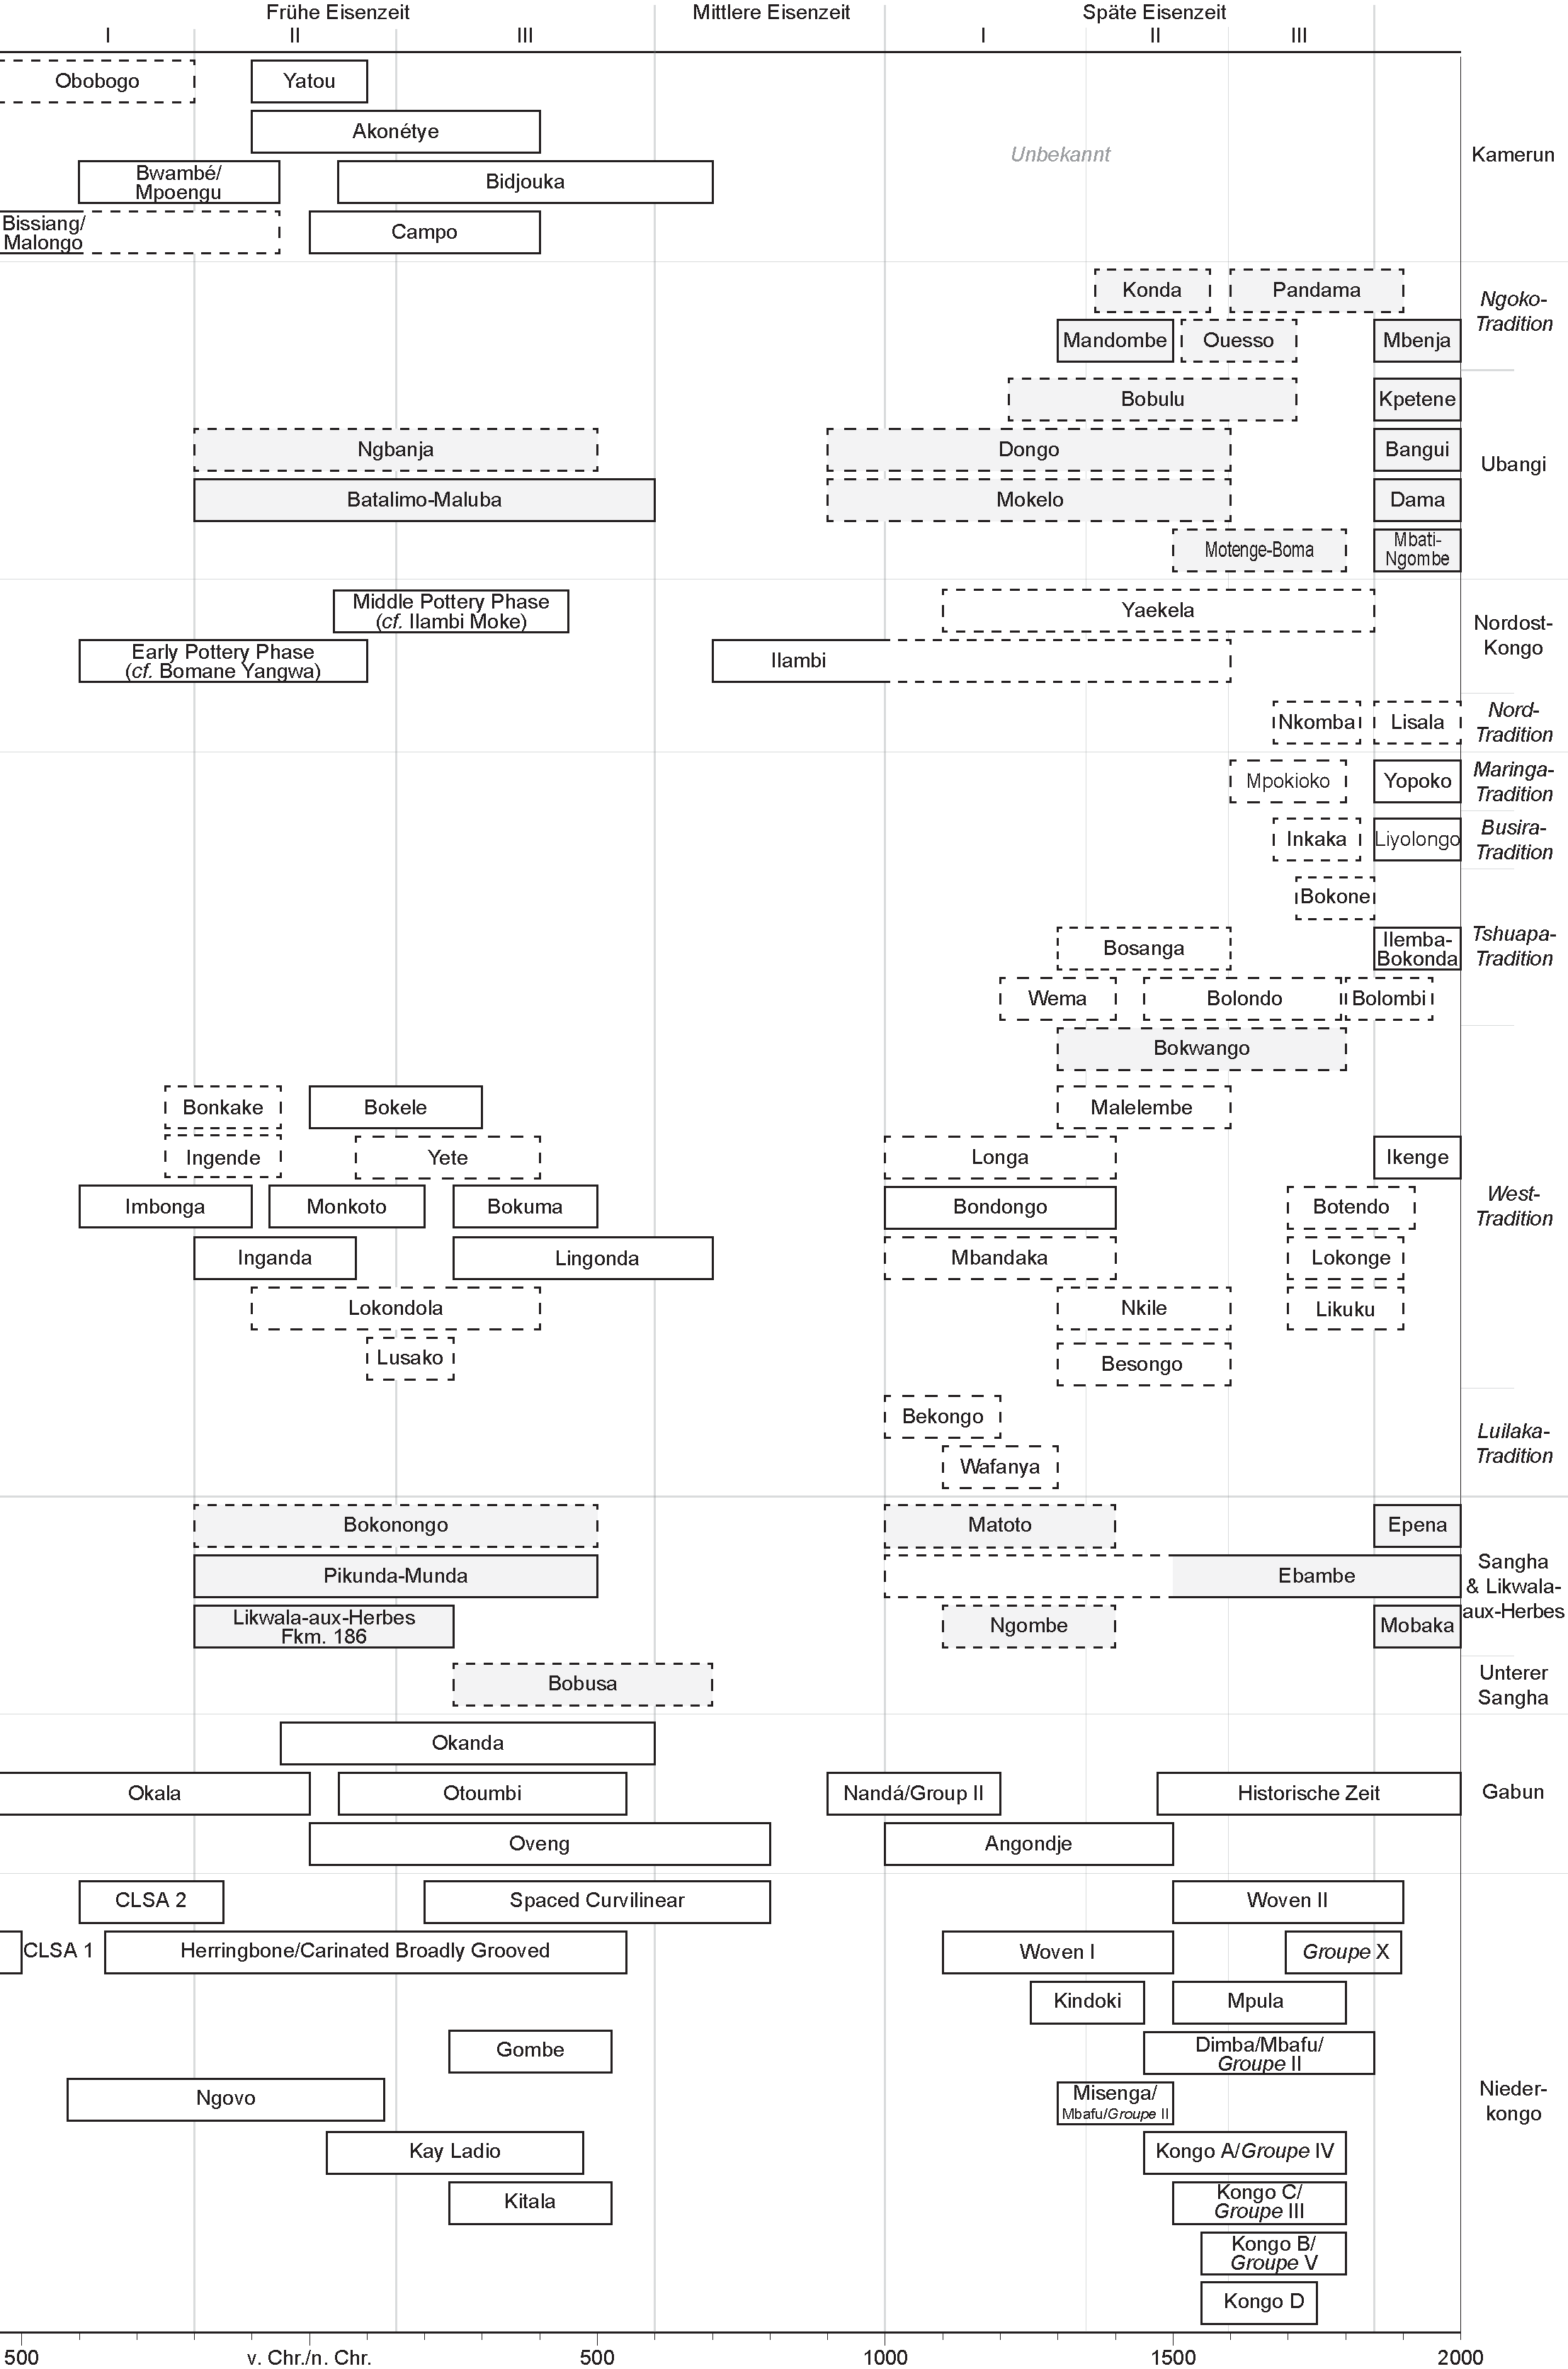
\includegraphics[height = .9\textheight]{fig/Chronologiesystem_v4.pdf}
	\caption{Chronologiesystem: Keramische Stilgruppen und Stiltraditionen (kursiv) ab 500 v.~Chr. Grau siehe Kap.~\ref{sec:Keramiksequenz}, Kamerun nach \textcites{Eggert.2006b}{Meister.2008b}{GouemGouem.20102011}{NlendNlend.20132014}, Nordostkongo nach \textcite{LivingstoneSmith.2017}, \textit{Nord-Tradition}~--~\textit{Luilaka-Tradition} nach \textcite{Wotzka.1995}, Gabun nach \textcites{Clist.20042005}{SanchezElipe.2015}{SanchezElipe.2016}, Niederkongo nach \textcites{deMaret.1982b}{deMaret.1982c}{deMaret.1986}{Gosselain.1988}{Denbow.2012}{Denbow.2014}{Cranshof.2018}{Clist.2018c}. Siehe Kap.~\ref{sec:Nachbarregionen}--\ref{sec:Zeitscheiben}.}
	\label{fig:Chronologiesystem}
	%\end{sidewaysfigure*}
\end{figure*}

%\subsection{Synchronisation}\label{sec:Synchronisation}
%\section{Synthese}

Der nachfolgende Abschnitt widmet sich der Zusammenführung der aus dem Arbeitsgebiet gewonnenen chronologischen Erkenntnisse mit den aus angrenzenden Regionen verfügbaren Informationen zum Besiedlungsgang. Zu diesem Zweck wurden die diskutierten Datierungsansätze der einzelnen Stile in ein Chronologiesystem übertragen (Abb.~\ref{fig:Chronologiesystem}). Es illustriert die Relation der keramischen Entwicklungen des Arbeitsgebiets zu den benachbarten Regionen. In der Übersicht beginnt die Auflistung der Regionen im nordwestlich gelegenen Kamerun, gefolgt vom nördlichen Bereich des Arbeitsgebietes sowie dem nordöstlichen und Inneren Kongobecken und endet im westlich des Arbeitsgebietes gelegen Gabun und im südwestlich gelegenen Niederkongo. Hieran schließt sich eine Besprechung dieser angrenzenden Großräume an. Sie folgt einer etwas anderen Sortierung, indem sie mit dem direkt an das Arbeitsgebiet angrenzenden, von \textsc{Wotzka} (1995) untersuchten Inneren Kongobecken beginnt.\footnote{Aus den folgenden Betrachtungen wurde der nördliche Teil des Arbeitsgebietes, der Südwesten der Zentralafrikanischen Republik weitestgehend ausgeklammert, da in dieser Region erst in jüngster Vergangenheit wieder Feldforschungen durchgeführt wurden (siehe Kap.~\ref{sec:FeldforschModern}). Einzig die Arbeitsgruppe um Karen \textcites{Lupo.2015}{Lupo.2018} erschloss systematisch neue Fundstellen im Ngotto-Waldschutzgebiet. Aufgrund der politischen Unruhen und des Bürgerkrieges seit Ende 2012 sind die in Bangui eingelagerten Funde nicht zugänglich. Während \textsc{Lupo} u.a. (ebd.) umfangreiche Serien von Radiokohlenstoffdatierungen vorlegt haben, können über die mit den Datierungen assoziierten Funde kaum Angaben gemacht werden.\label{ftn:Lupo2018}} In der grafischen Übersicht findet sich auf der unteren Achse eine absolutchronologische Skala, während an der oberen ein erster Entwurf einer kulturhistorischen Periodisierung aufgetragen ist (siehe Kap.~\ref{sec:Zeitscheiben}). Die im folgenden genannten Radiokohlenstoffdatierungen finden sich sämtlich im \textit{Archive des datations radiocarbones d’Afrique centrale} (aDRAC)-Online-Datenbank.\footnote{Siehe \url{https://github.com/dirkseidensticker/aDRAC} sowie \url{https://zenodo.org/record/61113} (Stand 03.\,10.\,2017).}